\documentclass[aspectratio=169,10pt]{beamer}
\usetheme{Berlin}
% https://www.overleaf.com/learn/latex/Beamer
\setbeamercovered{transparent}

\AtBeginSection[]{
  \begin{frame}
  \vfill
  \centering
  \begin{beamercolorbox}[sep=8pt,center,shadow=true,rounded=true]{title}
    \usebeamerfont{title}\insertsectionhead\par%
  \end{beamercolorbox}
  \vfill
  \end{frame}
}

\usepackage{graphicx}
\usepackage{pgfplots}
\pgfplotsset{compat=1.18}
\usepackage{hyperref, blindtext}
\usepackage{tikz, tikz-cd}

\title{A Coarse Introduction to Algebraic Geometry}
\author{A mini talk given on discord by .hchan}
\date{Oct 2026}

\begin{document}

\maketitle

\begin{frame}{Table of Contents}
    \tableofcontents
\end{frame}

\section{Quick Review}

\begin{frame}{Rings}
    \begin{block}{Definition}
        A \textit{ring} is a set $R$ with two binary operations $+$ and $\cdot$ such that
        \begin{itemize}
            \item $(R,+)$ is an abelian group with identity $0$,
            \item $(R,\cdot)$ is associative and commutative, with identity $1$,
            \item $a(b+c) = ab + ac$ for all $a,b,c \in R$.
        \end{itemize}
        A \textit{ring homomorphism} $\varphi : R \to S$ preserves $+$, $\cdot$ and $1$.
    \end{block}
    \begin{block}{Definition}
        An \textit{ideal} of $R$ is an additive subgroup $I \subseteq R$ such that $rI \subseteq I$ for all $r \in R$. It is \textit{maximal} if $I \neq R$ and no ideal lies strictly between $I$ and $R$.
    \end{block}
\end{frame}

\begin{frame}{Rings (cont.)}
    \begin{block}{Definition}
        If $I \subseteq R$ is an ideal, the \textit{quotient ring} $R/I$ is the set of cosets $a + I$, with
        \[
            (a+I) + (b+I) = (a+b) + I, \qquad (a+I)(b+I) = ab + I.
        \]
        These operations are well defined precisely because $I$ is an ideal.
    \end{block}
    \begin{theorem}[First Isomorphism Theorem]
        If $\varphi : R \to S$ is a ring homomorphism, then $\ker \varphi$ is an ideal of $R$, and
        \[
            R / \ker \varphi \;\cong\; \operatorname{im} \varphi.
        \]
    \end{theorem}
\end{frame}

\begin{frame}{Topologies}
    \begin{definition}
        Let $X$ be a set. A \textit{topology} $\mathcal{T}$ on $X$ is a collection of subsets of $X$, called the \textit{open sets}, such that the following three properties are satisfied:
        
        \begin{enumerate}
            \item $\varnothing, X \in \mathcal{T}$.
            \item If $U_1, \dots, U_n \in \mathcal{T}$ then so is $\bigcap_{i=1}^{n} U_i$; i.e. ($\mathcal{T}$ is closed under \textit{finite intersection}).
            \item If $\{U_\alpha\}_{\alpha \in \Lambda} \subseteq \mathcal{T}$ then so is $\bigcup_{\alpha \in \Lambda} U_\alpha$; i.e. ($\mathcal{T}$ is closed under \textit{{\color{red}arbitrary} union}).
        \end{enumerate}
        For simplicity we will often refer to $X$ itself as a topological space.
    \end{definition}
\end{frame}

\section{Rings of Functions}

\begin{frame}{Rings of functions on a space}

Suppose that $X$ is a set and $R$ is any ring.
\vspace{12pt}

Then the set of all functions from $X$ to $R$ naturally inherits the structure of a ring, via $(f+g)(x) := f(x) +g(x)$ and $(f \cdot g)(x) = f(x)\cdot g(x)$.

The additive identity is the zero function and the multiplicative identity is the one function.
\vspace{12pt}

We may restrict this ring to only contain functions with specific properties, e.g. continuous, differentiable, when it makes sense.

We will call these rings \textit{rings of functions}.

\end{frame}

\begin{frame}{Rings of functions on a space (cont.)}

Often times we are interested in the cases where the functions have some additional structure. Indeed, it turns out that many areas of mathematics can be described as the study of certain rings of functions:

\begin{itemize}
    \item In point-set topology, we are interested in studying the ring of continuous functions on a topological space.
    \item In measure theory, we are interested in studying the ring of bounded measurable functions on $\mathbb{R}^n$.
    \item In differential geometry, we are interested in studying the ring of smooth (i.e. infinitely differentiable) functions on smooth manifolds.
    \item In complex analysis, we are interested in studying the ring of holomorphic (complex-differentiable) functions on $\mathbb{C}$.
    \item In algebraic geometry, we are interested in studying the ring of polynomial functions on ??? (We will answer what this is later).
\end{itemize}
\vspace{12pt}
\end{frame}


\begin{frame}{A first example}
\begin{example}
    Let us consider the ring of continuous real functions on $[0,1]$; i.e. $R = C([0,1])$.
    \vspace{12pt}
    
    If $p \in [0,1]$, let $\mathfrak{m}_p := \{f \in R : f(p) = 0\}$. It is easily verified that this is an ideal, and in fact a maximal ideal. This is known as the maximal ideal at $p$.
\end{example}

\begin{theorem}
    Every maximal ideal of $R$ is given by the maximal ideal at $p$ for some $p \in [0,1]$.
\end{theorem}
\end{frame}


\begin{frame}{A first example (cont.)}
\begin{proof}
    \renewcommand{\qedsymbol}{}
    Let $\mathfrak{m}$ be a maximal ideal of $R$. We proceed in 3 steps.
    \begin{enumerate}
        \pause
        \item If $f\in\mathfrak{m}$, then there must exist some $x \in [0,1]$ such that $f(x) = 0$.
        
        Indeed, if this is not true then $1/f$ is a continuous function on $[0,1]$, such that $f$ is a unit. But then no maximal ideal can contain a unit.
        \pause
        \item If $f,g \in \mathfrak{m}$, then $Z(f) \cap Z(g) \neq \varnothing$.

        Indeed, if this is not true then $f^2+g^2$ is nonzero everywhere and is a unit, which is not possible.
    \end{enumerate}
\end{proof}
\end{frame}

\begin{frame}{A first example (cont..)}
\begin{proof}[Proof (cont.)]
    \begin{enumerate}
        \setcounter{enumi}{2}
        \item There must exist $p \in [0,1]$ such that $f(p)=0$ for all $f \in \mathfrak{m}$.

        Indeed, if this is not true then for every $x$ we may find an $f_x$ such that $f_x(x) \neq 0$. By continuity we may find an open neighbourhood $U_x$ of $x$ on which $f_x$ is nonzero. Proceeding in this way we may find an open cover of $[0,1]$, and by compactness we obtain a finite subcover $\{U_i\}$.

        But then the element $\sum f_i^2 \in \mathfrak{m}$ is a unit, and we have reached a contradiction.
    \end{enumerate}
\end{proof}
\end{frame}


\begin{frame}{A Remark.}
The theorem is not true if you replace $[0,1]$ with $(0,1)$.

Indeed, let $I = \{f \in R : f \equiv 0 \text{ on some neighbourhood of }0\}$. This is a proper ideal that cannot be contained in $\mathfrak{m}_p$ for any $p$.

\begin{itemize}
    \item This tells us that not all topological spaces and not all rings of functions are well-suited for the algebro-geometric treatment. For those in the know, this is motivation for the  Zariski topology.
    \item This tells us that not all topological spaces and not all rings of functions are well-suited for the algebro-geometric treatment. This motivates the  Zariski topology which we will see later.
\end{itemize}
\end{frame}

\section{Building the Dictionary}

\begin{frame}[label=Quotients]{Quotients}
    Let us further build the dictionary between topological spaces and rings, and see what kind of topological properties or operations can be detected by its ring of functions.
    \vspace{12pt}

    Let $R_X$ be a ring of functions on some set $X$. If $S \subsetneq X$ is some nonempty subset, we may naturally obtain a ring of functions $R_S$ on $S$ by restricting the domain of the functions in $R_X$; whence a ring homomorphism $\pi: R_X \to R_S$ given by $f \mapsto f\vert_S$.

    \pause
    \begin{theorem}
        $R_S$ is isomorphic to the quotient of $R_X$ by the ideal $V(S) := \{f \in R_X : f \vert_S \equiv 0\}$.
    \end{theorem}

    \pause
    \begin{proof}
        $\pi$ is surjective by definition.

        Now suppose that $f \in \ker \pi$. Then $f\vert_S = \pi(f) = 0$. Conversely if $f \vert_S \equiv 0$ then $\pi(f) =0$.
    \end{proof}
\end{frame}

\begin{frame}{Connectedness}
    If $X$ is a topological space, we say that a subset of $X$ is \textit{disconnected} if it can be written as the union of two disjoint nonempty open sets $A,B$. In which case we may write $X = A \sqcup B$. The subset is said to be connected otherwise.

    Let $R_X$ denote the ring of continuous functions from $X$ to $\mathbb{R}$.

    \pause
    \begin{theorem}
        $X = A \sqcup B$ if and only if $R_X \simeq R_A \times R_B$.
    \end{theorem}

    \pause
    \begin{proof}
        $(\Rightarrow):$ Suppose that $X = A \sqcup B$. Let $f$ be the function that is $1$ on $A$ and $0$ on $B$. Then $R_X \simeq \langle f \rangle \times \langle 1-f \rangle$.
        
        $(\Leftarrow):$ Suppose that $R_X \simeq R_A \times R_B$. Let $f$ be the function that corresponds to $(1,0)$ under this isomorphism. Then $A = f^{-1} (1)$ and $B = f^{-1} (0)$.
    \end{proof}
\end{frame}


\begin{frame}{Irreducibility}
    If $X$ is a topological space, we say that a subset of $X$ is \textit{reducible} if it can be written as the union of two distinct nonempty proper closed sets $C,D$. It is said to be irreducible otherwise.

    Let $R_X$ denote the ring of continuous functions from $X$ to $\mathbb{R}$.
    \pause
    \begin{theorem}
        If $R_X$ has zero divisors, then $X$ is reducible.
    \end{theorem}

    \pause
    \begin{proof}
        Suppose that $fg=0$ with $f,g \neq 0$. Then $X = f^{-1}(0) \cup g^{-1}(0)$. Both sets are closed, and they are proper as neither $f$ nor $g$ is $0$ by assumption. They are distinct, as otherwise $X = f^{-1}(0) \cup g^{-1}(0) = f^{-1}(0)$, which forces $f = 0$.
    \end{proof}
\end{frame}


\begin{frame}{Dimension}
    There are various ways of defining what the dimension of a topological space is, of which I will not get into in this talk.
    \vspace{12pt}

    \pause
    For this example we will be considering two spaces. The space $\mathbb{R}^2$, which has topological dimension $2$, and the unit circle $S^1 = \{x^2+y^2=1\}$. Even though $S^1$ is inside $\mathbb{R}^2$, it actually has topological dimension $1$ as it can be parameterized with one variable (namely $(\cos(t), \sin(t))$). Let us consider the rings of polynomials on this space.
    \vspace{12pt}

    \pause
    We will approach this example with the following idea: let us try to count how many linearly independent polynomial functions of degree less than or equal to $d$ live on a space, and see how quickly that number grows with $d$.
\end{frame}

\begin{frame}{Dimension (cont.)}
    \begin{itemize}
        \item For the space $\mathbb{R}^2$, the functions of degree $\leq d$ are spanned by the monomials $x^a y^b$ with $a + b \leq d$.
        
        In total, this will give us $\sum_{i=0}^d (i+1) = \frac{1}{2} (d+1)(d+2)$. So the total number grows quadratically, and that tells us that the topological dimension of $\mathbb{R}^2$ is indeed $2$.

        \pause
        \item For the space $S^1 = \{x^2 + y^2 = 1\}$, because of \hyperlink{Quotients}{\textcolor{blue}{what we discussed earlier on quotients}}, the polynomial function $y^2$ is equivalent to $x^2-1$. So in fact the only monomials are of the form $x^a, x^a y$.

        In total, this will give us $(d+1) + d= 2d+1$ number of linearly independent functions. So the total number grows linearly, and that tells us that the topological dimension of $S^1$ is indeed $1$.
    \end{itemize}
\end{frame}


\begin{frame}{Smoothness}
    Suppose that $\gamma:\mathbb{R}\to\mathbb{R}^n$ is some (injective, regular) path in $\mathbb{R}^n$, and look at its image $\Gamma$.
        
    Then if $\gamma$ is not differentiable at some point, then the curve $\Gamma$ should have some kind of sharp bend at that point as well. It's clear that the converse is true as well.
    \vspace{12pt}
    
    \pause
    This tells us that we can detect the existence of sharp corners on the curve $\Gamma$ by seeing if $\gamma$ is differentiable or not. But then that is something that can be checked using functions on $\Gamma$:
        \begin{quote}
            The curve $\Gamma$ is smooth at a point $p$ $\iff$ for all $f:\mathbb{R}^n \to \mathbb{R}$, $f \circ \gamma$ is (infinitely) differentiable at $p$ if and only if $f$ is (infinitely) differentiable at $p$.
        \end{quote}

    \pause
    {\color{red}Warning.} The statement as described above is \textbf{not true}, and is only supposed to give informal intuition for how you could use rings of functions to determine smoothness. There is a rigourous formalism in which you can make this theorem true, but that is too much for me to get into here.
\end{frame}


\begin{frame}{Closed Sets}
    Let $X$ be a compact Hausdorff space. For a closed set $C \subseteq X$ and some subset $S \subseteq R_X$, define
    \[
        V(C) := \{f \in R_X : f|_C = 0\}, \qquad Z(S) := \{x\in X : f(x)=0 \text{ for all }f \in S\}.
    \]

    \pause
    \begin{theorem}
        If $C$ is closed, then $Z(V(C)) = C$.
    \end{theorem}

    \pause
    \begin{proof}
        Every $f \in V(C)$ vanishes on $C$, so $C \subseteq Z(V(C))$.
        
        Conversely, if $x \notin C$, by Urysohn's lemma there exists $f$ with $f|_C = 0$ and $f(x) = 1$.
    \end{proof}
\end{frame}

\begin{frame}{Ideals}
    Let $X$ be a compact Hausdorff space. For a closed set $C \subseteq X$ and some subset $S \subseteq R_X$, define
    \[
        V(C) := \{f \in R_X : f|_C = 0\}, \qquad Z(S) := \{x\in X : f(x)=0 \text{ for all }f \in S\}.
    \]

    \pause
    \begin{theorem}
        $Z(S) = Z(\langle S \rangle)$ for all $S$.
    \end{theorem}

    \pause
    \begin{proof}
        $Z(\langle S \rangle) \subseteq Z(S)$ follows immediately from the definition, since $S \subseteq \langle S \rangle$.

        Conversely, suppose that $f,g$ vanish on $Z(S)$. Then $(f+g)\vert_{Z(S)} = 0+0 =0$.
        
        For any $h \in R_X$, $(h \cdot f)\vert_{Z(S)} = h\vert_{Z(S)} \cdot 0 = 0$. Hence every element of $\langle S \rangle$ vanishes on $Z(S)$, i.e. $Z(S) \subseteq Z(\langle S \rangle)$.
    \end{proof}


\end{frame}

\begin{frame}{Closed set - ideal correspondence}
        \begin{theorem}
        $C \mapsto V(C)$ defines an injective, inclusion-reversing map from closed sets to ideals.
    \end{theorem}
    Hence proving facts about the ideals of $R$ will prove facts about the closed sets of $X$. This map is almost never surjective, however. For instance, when $X = [0,1]$, the principal ideals generated by $x$ and $x^2$ are distinct (as $x/x^2 = 1/x$ is not continuous at $0$) but share the same zero loci, namely $\{0\}$.

    \begin{itemize}
        \item For those in the know, this is exactly the issue that Hilbert's Nullstellensatz fixes. That theorem is the algebraic analogue of the $C([0,1])$ example we saw earlier, and how you prove that maximal ideals correspond to (closed) points in your topological space. This is the "correct" geometric interpretation of the Nullstellensatz.
        \item This problem will be fixed by the Nullstellensatz, which we will introduce later.
    \end{itemize}
\end{frame}


\section{The Pièce de Résistance}
\begin{frame}{Introduction}
    We have now seen that various topological properties can be detected by ring-theoretic properties of some corresponding ring of functions on that space. But that itself is not that impressive - why not just look at the original space itself? Why bother with rings of functions at all?
    \vspace{12pt}
    
    \pause As mentioned before, in algebraic geometry it turns out that we are only interested in polynomial (or rational) functions, as those are the only functions that can be well described by abstract algebra.
    \vspace{12pt}

    \pause Hence, for this example, we will take $R = \mathbb{R}[x,y]$, considered as a ring of polynomial functions on the vector space $\mathbb{R}^2$ in the natural way.

    Let our topological space $X$ be the graph of the parabola $y=x^2$.
    By our \hyperlink{Quotients}{\textcolor{blue}{previous discussion on quotients}}, we have that $R_X \simeq \mathbb{R}[x,y]/\langle y-x^2\rangle$. This is the space of all unique real-valued polynomial functions on $X$.
\end{frame}



\begin{frame}{A simple question}
  \centering
  \begin{tikzpicture}
  \begin{axis}[
    axis lines=middle,
    xmin=-2.5, xmax=2.5,
    ymin=-0.5, ymax=4.5,
    xtick=\empty, ytick=\empty,
    width=7cm, height=6cm,
    clip=false,
  ]
  \addplot[red, thick, domain=-2:2, samples=100] {x^2}
    node[pos=0.9, right, text=black] {$y=x^2$};
  \end{axis}
  \end{tikzpicture}

  \vspace{1em}
  How many times does the curve intersect the $x$-axis?

  \pause
  \vspace{0.5em}
  \visible<2->{There is one. This isn't a trick question.}
\end{frame}

\begin{frame}{Or is it?}
    \begin{center}
        
\includegraphics[width=0.6\textwidth, height=0.7\textheight]{VSauce.png}
    \end{center}
\end{frame}

\begin{frame}{The problem}
    \begin{itemize}
        \item The graph has two horizontal intercepts for every positive $y$-value. In other words, the "limit" of a line with two points on it is a line with a single point on it. That can't be right, $2$ shouldn't suddenly become $1$.
        \pause\item For those that know some linear algebra, you might recognize that what is happening is that the geometric multiplicity of the zero of the graph at $(0,0)$ is equal to $1$, but the algebraic multiplicity of the zero of the graph is equal to $2$.
        \pause\item In other words, even though the equation $x^2=0$ is saying that there should be two solutions at this point, there is physically not enough room in the graph for those two solutions to have separate points.
    \end{itemize}
\end{frame}

\begin{frame}{The fix}
\begin{columns}[T]
    \column{0.5\textwidth}
    \begin{itemize}
        \item Taking the horizontal intercept of the graph with the line $y=c$ is the same as restricting $X$ with the subspace $X \cap \{y=c\}$.
        \pause\item By \hyperlink{Quotients}{\textcolor{blue}{the discussion we had before}}, for the ring of polynomial functions this corresponds to the quotient map $(\mathbb{R}[x,y]/\langle y-x^2\rangle)/\langle y-c\rangle$.
        \pause\item When $c>0$, the ring is isomorphic to $\mathbb{R} \oplus \mathbb{R}$ which has two nonzero proper ideals, which tells you that there are exactly two closed sets in the intersection as we expect.
    \end{itemize}

    \column{0.5\textwidth}
    \centering
      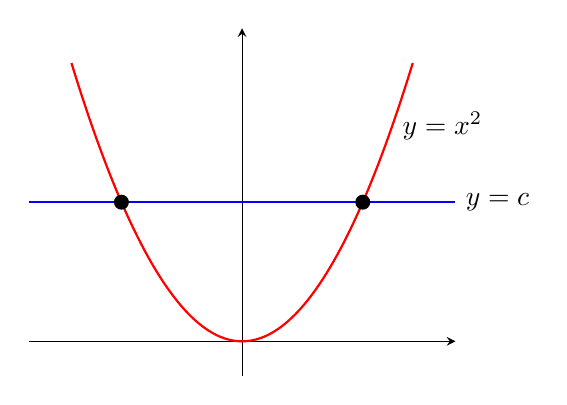
\begin{tikzpicture}
      \begin{axis}[
        axis lines=middle,
        xmin=-2.5, xmax=2.5,
        ymin=-0.5, ymax=4.5,
        xtick=\empty, ytick=\empty,
        width=7cm, height=6cm,
        clip=false,
      ]
      \addplot[red, thick, domain=-2:2, samples=100] {x^2}
        node[pos=0.9, right, text=black] {$y=x^2$};
      \addplot[blue, thick, domain=-2.5:2.5] {2}
        node[pos=1, right, text=black] {$y=c$};
      \addplot[only marks, mark=*, mark size=2.5pt, black]
        coordinates {(-1.4142,2) (1.4142,2)};
      \end{axis}
      \end{tikzpicture}
\end{columns}
\end{frame}

\begin{frame}{The fix (cont.)}
\begin{columns}[T]
    \column{0.7\textwidth}
    What happens now when $c=0$?
    \begin{itemize}
        \item By the third isomorphism theorem, the ring of polynomial functions is now isomorphic to $\mathbb{R}[x]/\langle x^2\rangle$.
        \pause\item This has one single nonzero proper ideal, which tells us there is one point of intersection.
        \pause\item But $\mathbb{R}[x]/\langle x^2\rangle$ is a dimension \textit{two} vector space over the real numbers, so the ring has \textit{remembered the fact that this point is supposed to have a "weight" of two}.
        \pause\item In other words, the ring of functions has managed to keep track of information about the space $X$ that $X$ itself is unable to remember. It somehow knows more about $X$ than $X$ knows about itself!
    \end{itemize}

    \column{0.3\textwidth}
      \centering
      \begin{tikzpicture}
      \begin{axis}[
        axis lines=middle,
        xmin=-1, xmax=1,
        ymin=-0.3, ymax=0.8,
        xtick=\empty, ytick=\empty,
        width=5cm, height=3.5cm,
        clip=false,
      ]
      \addplot[red, thick, dotted, domain=-0.5:0.5, samples=100] {x^2};
      \fill[black] (0,0) circle [radius=2pt];
      \end{axis}
      \end{tikzpicture}
\end{columns}
\end{frame}

\begin{frame}{But what does this mean?}
    As a real vector space, the ring $\mathbb{R}[x]/\langle x^2\rangle$ has a basis $\{1, \overline{x}\}$. Is there a way to figure out what this means?

    \begin{itemize}
        \item Recall that when $c>0$, we have that the ring of polynomials is isomorphic to $\mathbb{R}[x]/\langle x-\sqrt{c}\rangle \oplus \mathbb{R}[x]/\langle x+\sqrt{c}\rangle$.
        \pause\item This tells us that if you give me some unknown polynomial $f$; then knowing the values $f(\sqrt{c})$ and $f(-\sqrt{c})$ is exactly all the information you need to figure out what $f$ is on the intersection.
        \pause\item Following this interpretation, this is telling you that even at the single point $(0,0)$, you still need two pieces of information to be able to figure out what the unknown polynomial was on the intersection:
        \begin{itemize}
            \item Its actual value at the origin (i.e. $f(0)$); and
            \item the \textit{derivative} of the polynomial (i.e. $f'(0)$).
        \end{itemize}
    \end{itemize}
\end{frame}


\begin{frame}{But wait, there's more!}
\begin{columns}[T]
    \column{0.6\textwidth}
        What happens when $c<0$?

        \begin{itemize}
            \item The ring of polynomial functions is now isomorphic to $\mathbb{R}[x]/\langle x^2-c\rangle$, which is isomorphic to $\mathbb{C}$.
            \pause\item $\mathbb{C}$ has no nonzero proper ideals, so this tells us that there are zero points of intersection.
            \pause\item But $\mathbb{C}$ still has real dimension $2$, so it is saying that there \textit{still} should be two solutions!
            \pause\item The ring of polynomials has discovered the fact that our original graph was missing \textbf{the entire imaginary axis}, and $X$ is missing some solutions.
        \end{itemize}
    \column{0.4\textwidth}
  \centering
  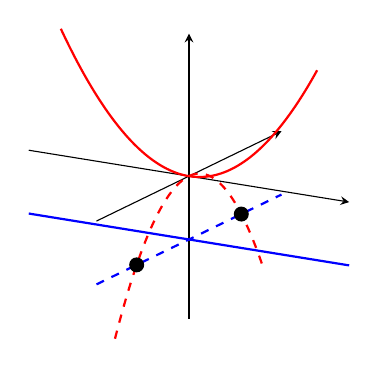
\begin{tikzpicture}
  \begin{axis}[
    view={30}{20},
    axis lines=center,
    xmin=-2.5, xmax=2.5,
    ymin=-2.5, ymax=2.5,
    zmin=-4.5, zmax=4.5,
    xtick=\empty, ytick=\empty, ztick=\empty,
    width=8cm, height=7cm,
    clip=false,
  ]
  % real parabola: x real
  \addplot3[red, thick, domain=-2:2, samples=100, samples y=0]
    ({x}, {0}, {x^2});
  % imaginary inputs: x = it gives y = -t^2
  \addplot3[red, thick, dashed, domain=-2:2, samples=100, samples y=0]
    ({0}, {x}, {-x^2});
  % y = c in the real plane (misses the real parabola)
  \addplot3[blue, thick, domain=-2.5:2.5, samples=2, samples y=0]
    ({x}, {0}, {-2});
  % y = c in the imaginary direction
  \addplot3[blue, thick, dashed, domain=-2.5:2.5, samples=2, samples y=0]
    ({0}, {x}, {-2});
  % intersections x = ±i sqrt(2)
  \addplot3[only marks, mark=*, mark size=2.5pt, black]
    coordinates {(0,1.4142,-2) (0,-1.4142,-2)};
  \end{axis}
  \end{tikzpicture}
\end{columns}
\end{frame}


% \section{Towards Varieties}

% \begin{frame}{The Zariski topology}
    
% \end{frame}

% \begin{frame}{The ideal correspondence}
    
% \end{frame}


% \begin{frame}{The Nullstellensatz}
% \end{frame}

% \begin{frame}{Affine varieties}
    
% \end{frame}

% \begin{frame}{A glimpse of the horizon}
    
% \end{frame}

\begin{frame}{What is Algebraic Geometry?}
\begin{columns}[T]
    \column{0.6\textwidth}
    \begin{itemize}
        \item Algebraic geometry is the study of the \textit{zero loci of systems of polynomials} using algebraic structures, mainly groups, rings, fields and modules.
        \pause\item Modern algebraic geometry is motivated by the philosophy that \textit{every} ring $R$ should be the ring of functions on some topological space (namely $\operatorname{Spec} R$, if you know what that is).
        \begin{itemize}
            \item The space $\operatorname{Spec} R$ is known as a \textit{scheme}, and was one of the twelve \href{https://en.wikipedia.org/wiki/Alexander_Grothendieck\#Major_mathematical_contributions}{``great ideas''} that Grothendieck contributed to the world of mathematics.
        \end{itemize}
    \end{itemize}

    \column{0.4\textwidth}
    \centering
    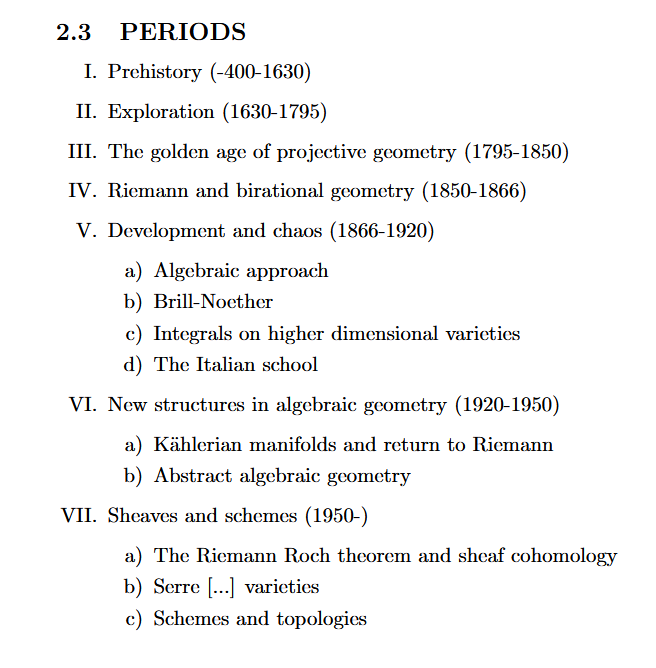
\includegraphics[width=\linewidth]{AG_history.png}\footnote[frame]{Image source: \url{https://arxiv.org/pdf/1803.00163}}
\end{columns}
\end{frame}

\begin{frame}{Any Questions?}
    \begin{center}
        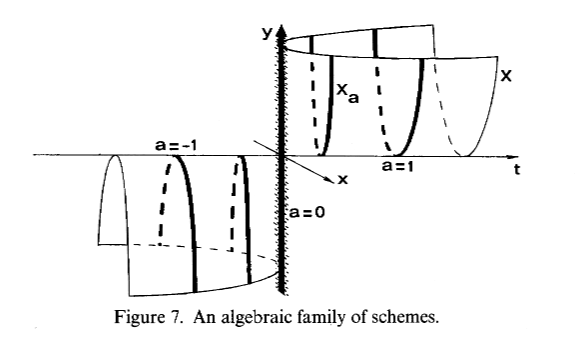
\includegraphics[width=0.5\linewidth]{family_of_schemes.png}
    \end{center}
\end{frame}


\end{document}